\chapter{Fourier Analysis -- Order in Complex Signals}
\label{chap:fourieranalyse}
\index{Fourier analysis}
\index{complex signals}

\subsection{Introduction: Hidden Order in Complex Signals}

\textbf{Guiding question:}
Can complex phenomena be decomposed into simple mathematical building blocks?

\medskip

When we look at the waveform of a piece of music,
it may at first appear chaotic and confusing.
Speech,
the sound of the sea,
light,
or technical radio signals also seem at first glance
like complicated patterns without any recognizable order.

Yet mathematics shows something remarkable:
behind many of these seemingly complex signals
there is an astonishingly simple mathematical structure\index{mathematical structure}.

A musical tone, for example, does not consist of a single vibration,
but of many superimposed frequencies.
Fourier analysis makes it possible
to reveal these individual components.

In this way, a complex signal
can be decomposed into simple periodic oscillations.
Mathematics therefore recognizes order
where initially only complexity seems visible.

\begin{DidacticBox}[What is a complex signal?]
	\small
	\label{box:fourier-komplexes-signal}
	A complex signal consists of many superimposed oscillations.
	
	A piano tone, for example, contains:
	
	\begin{itemize}
		\item a fundamental tone,
		\item numerous overtones,
		\item changes over time,
		\item small disturbances and background noises.
	\end{itemize}
	
	Nevertheless, Fourier analysis can mathematically decompose this structure
	and make the individual frequency components visible.
\end{DidacticBox}

The following figure first shows a complex signal,
as it might occur in a musical tone.
At first glance, the curve appears irregular.
In fact, however, it is composed of several simple oscillations.

% ============================================================
% Figure 1: Complex waveform of a tone
% ============================================================

\begin{figure}[h]
	\centering
	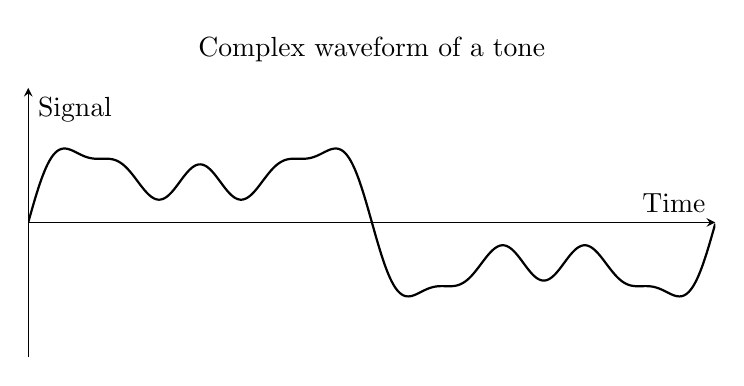
\begin{tikzpicture}
		\begin{axis}[
			width=0.85\textwidth,
			height=5cm,
			axis lines=middle,
			xlabel={Time},
			ylabel={Signal},
			xmin=0, xmax=6.28,
			ymin=-2.2, ymax=2.2,
			samples=500,
			domain=0:6.28,
			grid=both,
			xtick=\empty,
			ytick=\empty,
			title={Complex waveform of a tone}
			]
			\addplot[thick]
			{sin(deg(x)) + 0.6*sin(deg(3*x)) + 0.35*sin(deg(5*x)) + 0.2*sin(deg(9*x))};
		\end{axis}
	\end{tikzpicture}
	\caption{A complex signal initially appears confusing. However, it can be composed of several simple oscillations.}
	\label{fig:komplexe-wellenform}
\end{figure}

Fourier analysis conceptually decomposes this signal
into individual harmonic oscillations.
Each of these oscillations has its own frequency and its own strength.
Only their superposition produces the complex waveform.

% ============================================================
% Figure 2: Decomposition into individual sine waves
% ============================================================

\begin{figure}[h]
	\centering
	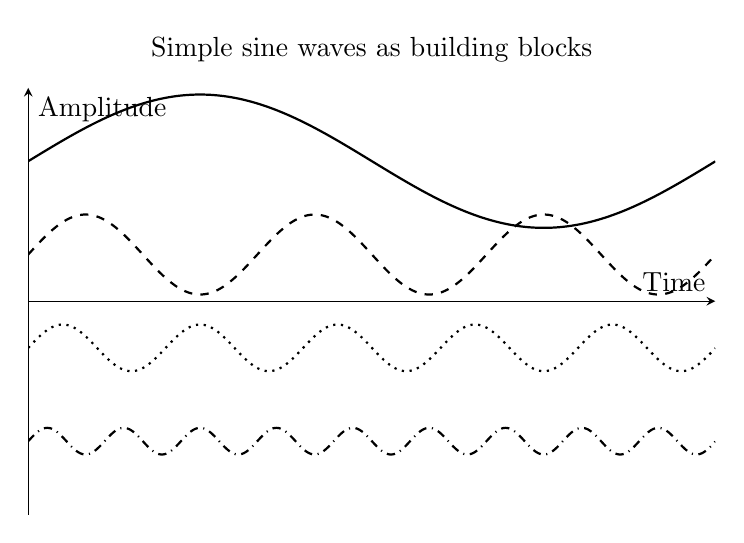
\begin{tikzpicture}
		\begin{axis}[
			width=0.85\textwidth,
			height=7cm,
			axis lines=middle,
			xlabel={Time},
			ylabel={Amplitude},
			xmin=0, xmax=6.28,
			ymin=-3.2, ymax=3.2,
			samples=400,
			domain=0:6.28,
			grid=both,
			xtick=\empty,
			ytick=\empty,
			title={Simple sine waves as building blocks}
			]
			\addplot[thick] {sin(deg(x)) + 2.1};
			\addplot[dashed, thick] {0.6*sin(deg(3*x)) + 0.7};
			\addplot[dotted, thick] {0.35*sin(deg(5*x)) - 0.7};
			\addplot[dashdotted, thick] {0.2*sin(deg(9*x)) - 2.1};
			
			\node[anchor=west] at (axis cs:6.35,2.1) {\small fundamental};
			\node[anchor=west] at (axis cs:6.35,0.7) {\small 3rd overtone};
			\node[anchor=west] at (axis cs:6.35,-0.7) {\small 5th overtone};
			\node[anchor=west] at (axis cs:6.35,-2.1) {\small 9th overtone};
		\end{axis}
	\end{tikzpicture}
	\caption{The individual sine waves are the mathematical building blocks of the complex signal. For better visibility, they are shown vertically shifted.}
	\label{fig:sinus-bausteine}
\end{figure}

In the frequency domain, it finally becomes visible
which frequencies are contained in the signal
and how strongly they occur.
The seemingly complicated waveform suddenly appears ordered.

% ============================================================
% Figure 3: Frequency spectrum
% ============================================================

\begin{figure}[h]
	\centering
	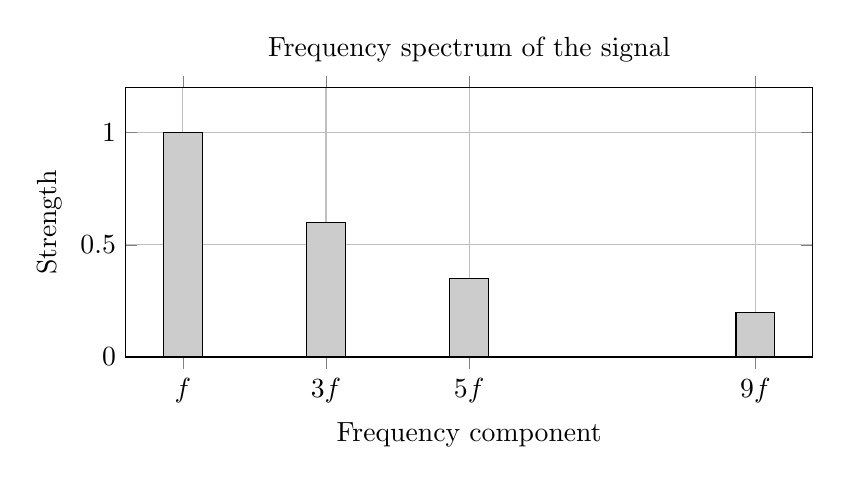
\begin{tikzpicture}
		\begin{axis}[
			width=0.85\textwidth,
			height=5cm,
			ybar,
			bar width=14pt,
			xlabel={Frequency component},
			ylabel={Strength},
			ymin=0, ymax=1.2,
			xtick={1,3,5,9},
			xticklabels={$f$,$3f$,$5f$,$9f$},
			grid=both,
			title={Frequency spectrum of the signal}
			]
			\addplot[
			fill=gray!40,
			draw=black
			]
			coordinates {
				(1,1.0)
				(3,0.6)
				(5,0.35)
				(9,0.2)
			};
		\end{axis}
	\end{tikzpicture}
	\caption{In the frequency domain, the hidden order of the signal becomes visible: a few frequency components determine its structure.}
	\label{fig:frequenzspektrum}
\end{figure}

The original complicated waveform suddenly appears ordered
in the frequency domain.
We immediately recognize
which frequencies dominate the signal
and how strong their respective contributions are.

Fourier analysis thus reveals a hidden mathematical structure
that was hardly recognizable in the original signal.
It shows, by example,
how mathematics can make order visible,
even when nature at first appears chaotic.

% ============================================================
\subsection{The Language of Oscillations}

Oscillations\index{oscillation} are among the most fundamental phenomena in nature.
A vibrating guitar string,
a water wave,
or an electromagnetic signal
changes periodically with time.

Especially important is the harmonic oscillation\index{harmonic oscillation}.
It is the simplest periodic motion
and occurs approximately wherever a system oscillates uniformly around an equilibrium position,
for example in a guitar string,
a pendulum,
or a tuning fork.

A typical harmonic oscillation can be written as

\[
y(t)=A\sin(2\pi f t+\varphi).
\]

Here:

\begin{itemize}
	\item $A$ is the amplitude\index{amplitude},
	\item $f$ is the frequency\index{frequency},
	\item $\varphi$ is the phase\index{phase},
	\item $t$ is time.
\end{itemize}

The frequency specifies
how often an oscillation repeats per second.
The unit of frequency is the hertz\index{hertz} (Hz).

The amplitude describes the strength of the oscillation.
For a sound, it corresponds for example to loudness.

The phase specifies
where the oscillation is within its periodic motion.
Two signals can have the same frequency
but be shifted in time relative to each other.

\begin{DidacticBox}[What does ``harmonic oscillation'' mean?]
	\small
	\label{box:fourier-harmonische-schwingung}
	A harmonic oscillation is the simplest possible periodic motion.
	
	It has a smooth,
	regular form
	and repeats continuously.
	
	Sine and cosine functions describe such motions particularly well.
	That is why they form the mathematical basis of Fourier analysis.
\end{DidacticBox}

% ============================================================
% Figure 1: Low and high frequency
% ============================================================

Frequency determines
how quickly an oscillation repeats.
A low frequency has only a few oscillations per time interval,
whereas a high frequency has many.

\begin{figure}[h]
	\centering
	\begin{tikzpicture}
		\begin{axis}[
			width=0.85\textwidth,
			height=6.5cm,
			axis lines=middle,
			xlabel={Time},
			ylabel={Amplitude},
			xmin=0, xmax=10,
			ymin=-2.6, ymax=2.8,
			samples=500,
			grid=both,
			xtick=\empty,
			ytick=\empty,
			title={Low and high frequency}
			]
			
			\addplot[thick]
			{sin(deg(x)) + 1.2};
			
			\addplot[dashed, thick]
			{sin(deg(3*x)) - 1.2};
			
			\node[anchor=west] at (axis cs:10.2,1.2)
			{\small low frequency};
			
			\node[anchor=west] at (axis cs:10.2,-1.2)
			{\small high frequency};
			
		\end{axis}
	\end{tikzpicture}
	\caption{Frequency describes how quickly a periodic motion repeats.}
	\label{fig:frequenzvergleich}
\end{figure}

% ============================================================
% Figure 2: Different amplitudes
% ============================================================

The amplitude determines the strength of an oscillation.
Large amplitudes correspond to stronger deflections,
small amplitudes to weaker ones.

\begin{figure}[h]
	\centering
	\begin{tikzpicture}
		\begin{axis}[
			width=0.85\textwidth,
			height=6cm,
			axis lines=middle,
			xlabel={Time},
			ylabel={Amplitude},
			xmin=0, xmax=10,
			ymin=-3, ymax=3,
			samples=500,
			grid=both,
			xtick=\empty,
			ytick=\empty,
			title={Different amplitudes}
			]
			
			\addplot[thick]
			{2*sin(deg(x))};
			
			\addplot[dashed, thick]
			{0.7*sin(deg(x))};
			
			\node[anchor=west] at (axis cs:10.2,2)
			{\small large amplitude};
			
			\node[anchor=west] at (axis cs:10.2,0.7)
			{\small small amplitude};
			
		\end{axis}
	\end{tikzpicture}
	\caption{Amplitude describes the strength of an oscillation.}
	\label{fig:amplitude}
\end{figure}

% ============================================================
% Figure 3: Phase shift
% ============================================================

The phase describes the temporal shift of an oscillation.
Two signals can have the same frequency
but be shifted in time relative to each other.

\begin{figure}[h]
	\centering
	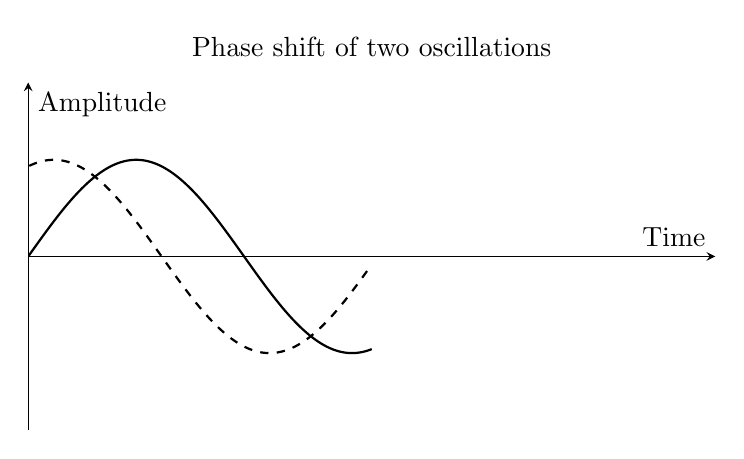
\begin{tikzpicture}
		\begin{axis}[
			width=0.85\textwidth,
			height=6cm,
			axis lines=middle,
			xlabel={Time},
			ylabel={Amplitude},
			xmin=0, xmax=10,
			ymin=-1.8, ymax=1.8,
			samples=500,
			grid=both,
			xtick=\empty,
			ytick=\empty,
			title={Phase shift of two oscillations}
			]
			
			\addplot[thick]
			{sin(deg(x))};
			
			\addplot[dashed, thick]
			{sin(deg(x+1.2))};
			
			\node[anchor=west] at (axis cs:10.2,0.8)
			{\small original oscillation};
			
			\node[anchor=west] at (axis cs:10.2,-0.8)
			{\small phase-shifted oscillation};
			
		\end{axis}
	\end{tikzpicture}
	\caption{Two oscillations with the same frequency but different phase.}
	\label{fig:phase}
\end{figure}

\begin{MathBox}[The sine function as a building block]
	\small
	\label{box:fourier-sinus-grundbaustein}
	In Fourier analysis, sine and cosine functions
	play a special role.
	
	They are mathematically simple,
	periodic,
	and have stable properties under differentiation and integration.
	
	This makes them ideal fundamental building blocks of complex signals.
\end{MathBox}

Sine and cosine functions occur frequently in nature
because many physical systems oscillate approximately harmonically
when their displacements are small.
This is why these functions play a central role in physics and engineering.

Fourier analysis ultimately examines not only the time evolution of an oscillation,
but also its frequency components.
This produces the so-called frequency spectrum\index{frequency spectrum}.

The frequency spectrum can be imagined
as the decomposition of a piece of music into individual tones.
Instead of viewing the entire signal at once,
the spectrum shows
which individual frequencies are hidden within it.

It therefore shows
which frequencies are contained in a signal
and how strong their respective contributions are.

This makes visible
that even complicated signals are often built from only a few fundamental oscillations.

% ============================================================
\subsection{Superposition: How Complex Signals Arise}

In reality, pure sine waves rarely occur in isolation.
Usually, many different frequencies are superimposed at the same time.

A musical tone, for example, does not consist only of a single fundamental tone,
but also of numerous overtones.
These determine the characteristic timbre of an instrument.

This produces a complex signal
that can nevertheless be described mathematically as a sum of simple oscillations.

Speech,
the sound of the sea,
and technical radio signals also arise
from the superposition of many different frequency components.

\medskip

The idea of superposition can be understood with a simple example.
If two stones are thrown into calm water,
two circular waves spread out.
When these waves meet,
their displacements add.

At some points the waves reinforce each other,
while at other points they weaken each other.
A rich pattern emerges,
although each individual wave is very simple on its own.

Complex sound signals arise in a very similar way.

\begin{DidacticBox}[Superposition of waves]
	\small
	\label{box:fourier-ueberlagerung-wellen}
	When several oscillations occur at the same time,
	their instantaneous displacements add.
	
	This superposition is called superposition\index{superposition}.
	
	Complex signals therefore often arise
	from the combination of many simple oscillations.
\end{DidacticBox}

In a piano, for example, not only the fundamental tone of a string is heard.
In addition, numerous overtones\index{overtone} with higher frequencies arise.

A flute,
a violin,
or the human voice
each has a different mixture of such frequency components.
That is why every instrument sounds characteristic,
even when the same fundamental tone is played.

The difference between two instruments
that play the same fundamental tone
therefore lies not in the fundamental tone alone,
but in the composition of the additional overtones.
Fourier analysis makes this hidden structure visible.

Human speech also arises through complex superpositions.
When speaking, the vocal cords,
the oral cavity,
and the tongue generate a constantly changing frequency pattern.

Even seemingly chaotic sounds such as ocean noise or wind
ultimately consist of a large number of superimposed frequencies.

% ============================================================
% Figure 1: Superposition of two waves
% ============================================================

The following figure shows
how two simple oscillations
combine by superposition to form a more complex signal.

\begin{figure}[h]
	\centering
	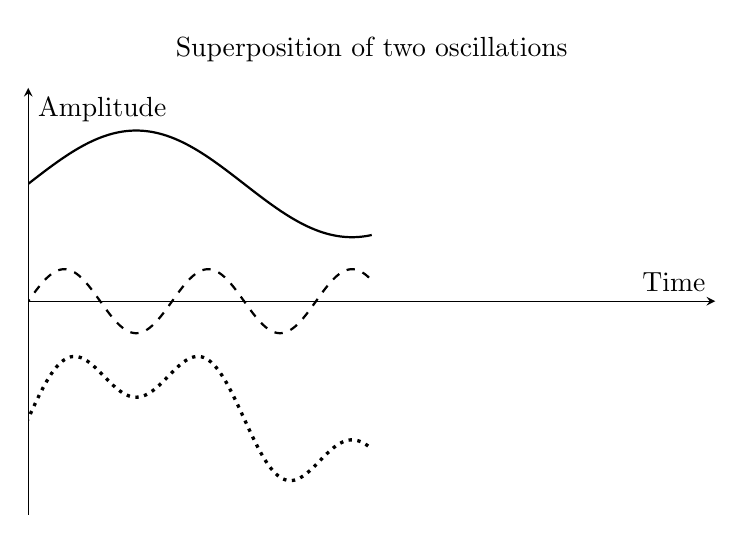
\begin{tikzpicture}
		\begin{axis}[
			width=0.85\textwidth,
			height=7cm,
			axis lines=middle,
			xlabel={Time},
			ylabel={Amplitude},
			xmin=0, xmax=10,
			ymin=-4, ymax=4,
			samples=500,
			grid=both,
			xtick=\empty,
			ytick=\empty,
			title={Superposition of two oscillations}
			]
			
			% first oscillation
			\addplot[thick]
			{sin(deg(x)) + 2.2};
			
			% second oscillation
			\addplot[dashed, thick]
			{0.6*sin(deg(3*x))};
			
			% sum
			\addplot[dotted, very thick]
			{sin(deg(x)) + 0.6*sin(deg(3*x)) - 2.2};
			
			\node[anchor=west] at (axis cs:10.2,2.2)
			{\small fundamental};
			
			\node[anchor=west] at (axis cs:10.2,0)
			{\small overtone};
			
			\node[anchor=west] at (axis cs:10.2,-2.2)
			{\small superposition};
			
		\end{axis}
	\end{tikzpicture}
	\caption{Two simple oscillations combine by superposition to form a more complex signal.}
	\label{fig:ueberlagerung}
\end{figure}

The lower curve arises because
the displacements of the two upper oscillations
are added at each point in time.

Regions with displacements in the same direction reinforce each other,
whereas opposite displacements partially cancel.

Even a few simple oscillations
can therefore produce a much more complex curve.

Mathematics thus shows
that complex signals often consist of surprisingly simple building blocks.

This decomposition of complex signals
into simple oscillations
forms the foundation of Fourier analysis.

Fourier analysis therefore shows
that even seemingly chaotic structures
are often built from simple mathematical patterns.

% ============================================================
\subsection{Joseph Fourier and the Great Idea}

At the beginning of the 19th century, the French mathematician
Joseph Fourier\index{Fourier, Joseph} studied a physical problem:
the propagation of heat\index{heat conduction}.

He investigated
how temperature changes in solid bodies,
how metal rods cool down,
and how heat spreads through the Earth.

This led to a surprising question:

\begin{NoteBox}[The starting point of Fourier analysis]
	\small
	\label{box:fourier-ausgangspunkt-waermeleitung}
	How can complicated temperature distributions be described mathematically?
\end{NoteBox}

Fourier recognized
that even very complicated distributions
can be represented by the superposition of simple periodic oscillations.

This idea was revolutionary.

Until then, many mathematicians believed
that only especially smooth and regular curves
could be described by trigonometric functions.

Fourier, however, claimed:
Even angular,
complicated,
or seemingly discontinuous functions
can be represented as sums of simple sine and cosine functions.

Today this statement appears natural.
At the time, it was highly controversial.

Many of his contemporaries initially considered Fourier's approach mathematically questionable.
How could an angular or discontinuous curve
be composed of smooth sine functions?

Only later did mathematicians recognize
how profound Fourier's idea really was.

\begin{HistoryBox}[Joseph Fourier]
	\small
	\label{box:fourier-joseph-fourier}
	Joseph Fourier (1768--1830) originally developed his theory
	while studying heat conduction.
	
	His ideas, however, reached far beyond this field
	and later influenced physics,
	electrical engineering,
	signal processing,
	astronomy,
	and quantum mechanics.
	
	Today, Fourier theory is one of the most important mathematical tools
	in modern science.
\end{HistoryBox}

The central statement of Fourier theory\index{Fourier theory} is:
Every periodic function can, under suitable conditions, be represented as a superposition
of sine and cosine functions.

This statement means
that even complicated structures
are often composed of simple periodic building blocks.

A plucked guitar string,
a speech signal,
or a digital audio signal
initially appears complex.

Fourier analysis shows, however,
that a mathematical order is hidden behind these signals.

\begin{DidacticBox}[Why Fourier's idea was revolutionary]
	\small
	\label{box:fourier-revolutionaere-idee}
	Fourier showed
	that complex curves do not have to be random or chaotic.
	
	Even complicated curves can be reduced
	to simple mathematical oscillations.
	
	This created an entirely new way of looking
	at signals,
	waves,
	and physical processes.
\end{DidacticBox}

A particularly striking example is the so-called square wave\index{square wave}.
It has abrupt jumps and sharp transitions
and therefore at first seems completely incompatible
with smooth sine functions.

Fourier theory shows, however,
that even such a signal
can be approximated by the superposition of harmonic oscillations.

% ============================================================
% Figure: Square wave and Fourier approximation
% ============================================================

\begin{figure}[h]
	\centering
	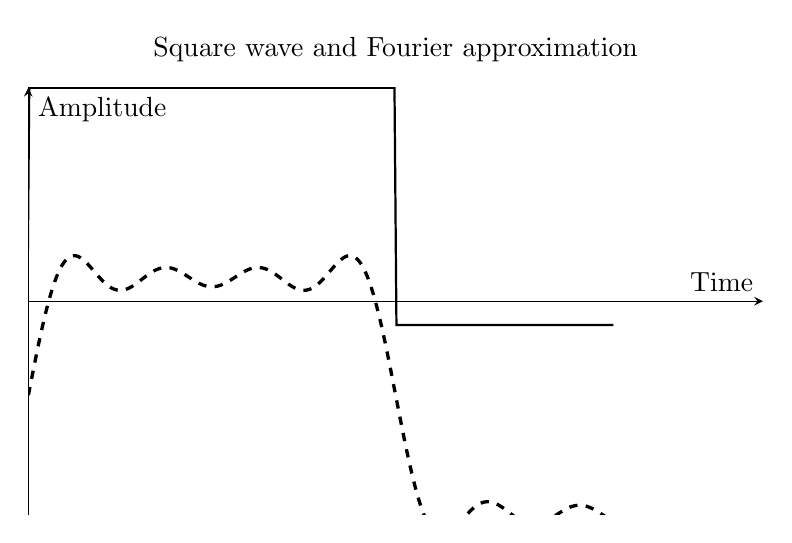
\begin{tikzpicture}
		\begin{axis}[
			width=0.9\textwidth,
			height=7cm,
			axis lines=middle,
			xlabel={Time},
			ylabel={Amplitude},
			xmin=0, xmax=6.28,
			ymin=-1.8, ymax=1.8,
			samples=600,
			grid=both,
			xtick=\empty,
			ytick=\empty,
			title={Square wave and Fourier approximation}
			]
			
			% square wave
			\addplot[
			thick
			]
			{sign(sin(deg(x))) + 0.8};
			
			% Fourier approximation
			\addplot[
			dashed,
			very thick
			]
			{
				(4/pi) * (
				sin(deg(x))
				+ (1/3)*sin(deg(3*x))
				+ (1/5)*sin(deg(5*x))
				+ (1/7)*sin(deg(7*x))
				)
				- 0.8
			};
			
			\node[anchor=west] at (axis cs:6.4,0.8)
			{\small ideal square wave};
			
			\node[anchor=west] at (axis cs:6.4,-0.8)
			{\small Fourier approximation};
			
		\end{axis}
	\end{tikzpicture}
	\caption{Even an angular square wave can be approximated by the superposition of several sine waves.}
	\label{fig:rechteck-fourier}
\end{figure}

The dashed curve shows
how several harmonic oscillations together
produce a signal
that already resembles the square wave remarkably well.

This makes visible
how powerful Fourier's idea really was:
Even seemingly irregular or abrupt structures
can be traced back to simple mathematical oscillations.

\begin{NoteBox}[Further exploration: square wave]
	\small
	\label{box:fourier-vertiefung-rechtecksignal}
	The square wave is a particularly vivid example of Fourier analysis:
	A discontinuous, angular function can be composed of smooth sine waves.
	The complete derivation of the corresponding Fourier series is given in
	Appendix~A, Section~\ref{sec:anhang_fourieranalyse_rechtecksignal}.
\end{NoteBox}

Fourier analysis originally arose from the study of heat conduction.
Later, however, it developed into a universal tool:
today it is used in acoustics, signal processing, quantum mechanics,
image compression, and digital communication.

% ============================================================
\subsection{From the Time Domain to the Frequency Domain}

In everyday life, we usually view signals in the time domain\index{time domain}.
We examine
how a signal changes over time.

A music signal, for example,
appears as a complicated waveform
whose shape changes constantly.

Fourier analysis, however, allows an entirely different perspective:
Instead of looking only at the time evolution,
we analyze the frequencies contained in the signal.

This produces the so-called frequency domain\index{frequency domain}.

\medskip

This shift in perspective is of central importance.

In the time domain, we see
how a signal evolves.

In the frequency domain, by contrast, we recognize
which oscillations the signal is composed of.

This can be imagined in a way similar to a piece of music:
While in the time domain we perceive only the overall sound,
the frequency domain shows
which individual tones and overtones are contained in it.

% ============================================================
% Figure: Time domain and frequency domain
% ============================================================

\begin{figure}[h]
	\centering
	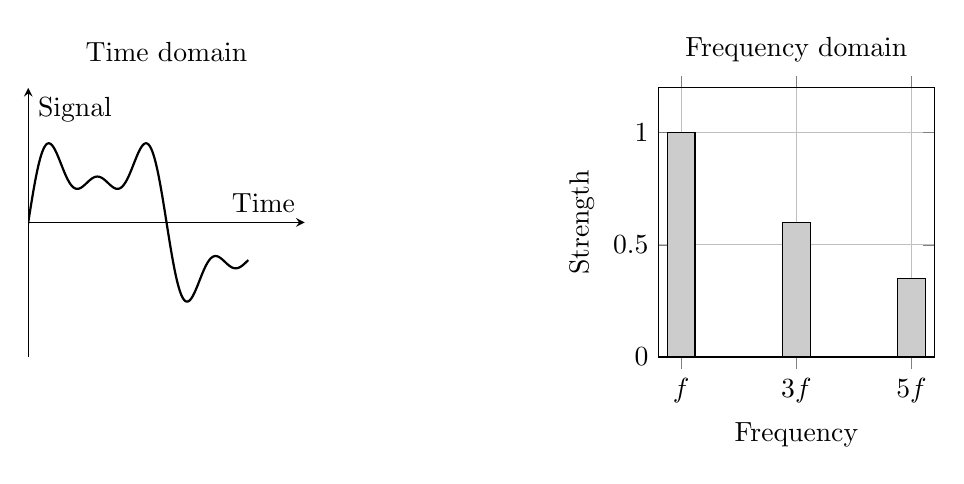
\begin{tikzpicture}
		
		% --------------------------------------------------------
		% Time domain
		% --------------------------------------------------------
		
		\begin{axis}[
			width=0.42\textwidth,
			height=5cm,
			at={(0cm,0cm)},
			axis lines=middle,
			xlabel={Time},
			ylabel={Signal},
			xmin=0, xmax=6.28,
			ymin=-2.2, ymax=2.2,
			samples=500,
			grid=both,
			xtick=\empty,
			ytick=\empty,
			title={Time domain}
			]
			
			\addplot[
			thick
			]
			{
				sin(deg(x))
				+ 0.6*sin(deg(3*x))
				+ 0.35*sin(deg(5*x))
			};
			
		\end{axis}
		
		\begin{axis}[
			width=0.42\textwidth,
			height=5cm,
			at={(8cm,0cm)},
			ybar,
			bar width=10pt,
			xlabel={Frequency},
			ylabel={Strength},
			ymin=0,
			ymax=1.2,
			xtick={1,3,5},
			xticklabels={$f$,$3f$,$5f$},
			grid=both,
			title={Frequency domain}
			]
			
			\addplot[
			fill=gray!40,
			draw=black
			]
			coordinates {
				(1,1.0)
				(3,0.6)
				(5,0.35)
			};
			
		\end{axis}
		
	\end{tikzpicture}
	\caption{
		On the left, the signal is shown in the time domain.
		On the right, the frequency domain shows
		which frequencies the signal is composed of.
	}
	\label{fig:zeit-frequenzbereich}
\end{figure}

Fourier analysis therefore not only decomposes a signal mathematically,
but also changes the way we look at the problem.

In the time domain, a signal often appears complicated and confusing.
In the frequency domain, however, simple and clearly recognizable patterns often emerge.

This allows hidden structures to be recognized
that would hardly be visible in the original signal.

Fourier analysis thus shows
that seemingly complex signals
often contain a hidden mathematical order.

\begin{NoteBox}[Time domain and frequency domain]
	\small
	\label{box:fourier-zeitbereich-frequenzbereich}
	The time domain describes
	how a signal changes over time.
	
	The frequency domain, by contrast, shows
	which frequencies are contained in the signal
	and how strong their respective contributions are.
	
	Fourier analysis connects both perspectives
	and thereby makes hidden structures visible.
\end{NoteBox}

\subsection{Applications of Fourier Analysis}

\subsubsection*{Music and Acoustics}
\phantomsection

Fourier theory plays a central role in modern music technology.

Electronic instruments such as synthesizers\index{synthesizer} or digital organs\index{digital organ}
produce sounds through electronic circuits or digital signal processing.

Different periodic waveforms are used,
such as sine,
square,
or sawtooth waves\index{sawtooth wave}.

By combining different frequencies,
complex timbres are produced.

Fourier theory mathematically describes
how such complex sounds
can be composed from simple oscillations.

This makes it understandable
why different instruments can sound completely different
even when they play the same pitch.

\medskip

Musical notation also has a mathematical foundation.
A note\index{note} does not merely stand for a sound,
but also for a certain pitch and a certain duration.

Pitch is physically connected to the frequency of an oscillation.
The higher the frequency,
the higher the perceived tone.
An octave\index{octave} corresponds to a doubling of the frequency:
\[
f \longrightarrow 2f.
\]

Musical intervals are also based on numerical ratios.
A fifth\index{fifth} can be described approximately by the frequency ratio
\[
\frac{3}{2},
\]
and a fourth\index{fourth} by
\[
\frac{4}{3}.
\]

In modern equal temperament, the octave is divided into twelve equal semitone steps\index{semitone steps}.
The frequency factor between two adjacent semitones\index{semitone} is therefore
\[
2^{1/12}.
\]

This shows:
musical notes\index{musical note} are not merely cultural signs,
but refer to a mathematical order of frequencies,
time relationships, and oscillatory structures.

\begin{NoteBox}[Musical notes as mathematical order]
	\small
	\label{box:Musiknoten}
	A musical note describes not only a sound,
	but also mathematical properties:
	pitch, duration, rhythm, and frequency ratios.
	
	The octave corresponds to a doubling of frequency,
	and musical intervals are based on numerical ratios.
	Thus even musical notation shows
	that music has a mathematical structure.
\end{NoteBox}

Synthesizers use exactly this principle:
they combine different waveforms and frequencies
to create artificial sounds.
Fourier theory provides the mathematical description
of how complex sound structures arise from simple periodic oscillations.

% ------------------------------------------------------------
\subsubsection*{Image and Signal Processing}
\phantomsection

Fourier analysis is used not only for tones and oscillations,
but also for images\index{image processing}.

At first this is surprising,
because an image does not seem to have anything to do with oscillations.
Mathematically, however, an image can be understood as a distribution of brightness
and color.

Slow changes in brightness correspond to low spatial frequencies\index{spatial frequency}.
These include large areas,
soft transitions,
and coarse shapes.

Sharp edges,
fine details,
or image noise correspond to high spatial frequencies.

\begin{DidacticBox}[Frequencies in images]
	\small
	\label{box:fourier-frequenzen-in-bildern}
	In sounds, frequency describes
	how quickly an oscillation changes over time.
	
	In images, a spatial frequency describes
	how quickly brightness or color changes across the image.
	
	Large smooth areas have low frequencies,
	while fine details and edges have high frequencies.
\end{DidacticBox}

This principle is the basis of many image-processing methods.

In JPEG compression\index{JPEG compression}, image information is rearranged
so that less important details can be reduced more strongly.
The human eye often perceives fine changes in certain image components
less clearly.
This makes it possible to reduce the amount of data substantially
without making the image look significantly worse at first glance.

Frequency analysis also plays an important role in noise reduction\index{noise reduction}.
Noise often appears as a fine,
irregular pattern.
Such components often lie in the range of higher frequencies
and can be selectively weakened.

Conversely, edges and fine structures can be emphasized
by amplifying high-frequency components.
In this way, images can be sharpened
or certain patterns made more visible.

However, undesirable effects can also occur at sharp edges.
Particularly abrupt brightness jumps cannot be represented perfectly
by Fourier approximations.

Small over- or undershoots then occur,
which are known as the Gibbs phenomenon\index{Gibbs phenomenon}.

Such effects occur, among other places,
in image compression,
signal filtering,
and digital audio methods.

\begin{DidacticBox}[The Gibbs phenomenon]
	\small
	\label{box:fourier-gibbs-phaenomen}
	When abrupt jumps or sharp edges
	are approximated by Fourier series,
	characteristic overshoots occur
	near these transitions.
	
	This behavior is called the Gibbs phenomenon.
\end{DidacticBox}

The following figure shows the typical overshoot
of a Fourier approximation at a sudden change in a signal.
The more Fourier components are used,
the smoother the regions between the jumps become.
However, the overshoots at the jump discontinuities remain characteristic.

% ============================================================
% Figure: Gibbs phenomenon
% ============================================================
\begin{figure}[h]
	\centering
	\includegraphics[width=0.95\textwidth]{Bilder/gibbs-en.png}
	\caption{The Gibbs phenomenon: A Fourier approximation of a square wave shows characteristic over- and undershoots at the jump discontinuities.}
	\label{fig:gibbs-bild}
\end{figure}

Even when more and more Fourier components are used,
the overshoot at the jump discontinuity does not disappear completely.

The Gibbs phenomenon thus shows
that the mathematical approximation of sharp transitions
has fundamental limits.

Similar overshoot effects also occur in real physical systems.
In fast switching processes in electronic circuits,
for example in transistors or digital signals,
short ringing effects or voltage spikes often appear.

Mathematics therefore describes not only an abstract phenomenon,
but also explains real effects in modern technology.

Many image-processing methods are based on
amplifying,
weakening,
or removing certain frequency components.
In this way, images can be compressed,
denoised,
sharpened,
or analyzed.

Fourier analysis therefore shows
that visual information also possesses a hidden mathematical structure.
An image is not merely a collection of pixels,
but can be understood as an interplay of spatial patterns.

% ------------------------------------------------------------
\subsubsection*{Medical Applications}
\phantomsection

Fourier analysis also plays a central role in modern medicine.

Many medical measurement methods do not initially produce direct images,
but complex signals
that must be evaluated mathematically.

Only through the analysis of these signals
can hidden structures of the body be made visible.

\medskip

A particularly well-known example is magnetic resonance imaging\index{magnetic resonance imaging} (MRI\index{MRI}).

Initially, electromagnetic measurement signals are produced
that contain information about the inside of the body.
Only with the help of mathematical methods,
including Fourier analysis,
can detailed cross-sectional images be reconstructed from them.

Mathematics thus becomes a tool
that makes invisible structures of the body visible.

\begin{PhysicsBox}[Mathematics makes the body visible]
	\small
	\label{box:fourier-medizinische-bildgebung}
	Modern medical imaging is often not based on direct photographs,
	but on the mathematical analysis of complex signals.
	
	Fourier analysis helps reconstruct images and structures of the body
	from these measurement data.
\end{PhysicsBox}

Frequency analysis also plays an important role
in the study of brain activity.

In an electroencephalogram\index{electroencephalogram} (EEG\index{EEG}),
electrical voltages are measured at the surface of the head.
These signals consist of different frequency components
that are associated with different activity states of the brain.

For example, one distinguishes:

\begin{itemize}
	\item alpha waves\index{alpha waves} (relaxed wakefulness),
	\item beta waves\index{beta waves} (active concentration),
	\item theta waves\index{theta waves} (sleep and relaxation states).
\end{itemize}

By analyzing these frequency patterns,
characteristic brain activities can be recognized
that would often be difficult to see in the pure time signal.

Ultrasound methods\index{ultrasound} also use principles of signal and frequency analysis.

Reflected sound waves are examined
to obtain information about tissue,
organs,
or blood flow.

Many medical procedures initially measure only signals or waves.
Only the mathematical analysis of these data
turns them into understandable images or diagnostic information.
Fourier analysis thereby directly connects mathematics,
physics,
and modern medicine.

Fourier analysis therefore shows impressively
that mathematics does not merely describe abstract formulas,
but helps make hidden structures of the human body visible.

% ------------------------------------------------------------
\subsubsection*{Physics and Astronomy}
\phantomsection

In physics, Fourier analysis makes it possible to study complex wave phenomena.

Many physical processes can be described as superpositions of waves.
Fourier theory helps analyze these structures mathematically
and makes hidden frequency components visible.

\medskip

A particularly important example is the spectral analysis\index{spectral analysis} of light.

White light initially appears uniform to the human eye.
In fact, however, it consists of many different wavelengths or frequencies.

Using a prism or a spectrometer,
light can be decomposed into its individual color components.

Certain chemical elements absorb or emit very characteristic frequencies.
This produces so-called spectral lines\index{spectral lines}.

Astronomers can thereby determine
which chemical elements are present in stars or galaxies,
even though these objects are unimaginably far away.

\begin{PhysicsBox}[Spectral lines as mathematical signatures]
	\small
	\label{box:fourier-spektrallinien-signatur}
	Every chemical element has characteristic spectral lines.
	
	By analyzing the frequencies of emitted or absorbed light,
	one can determine
	which elements are present in a star.
	
	Mathematics thus becomes a tool
	for obtaining information about distant objects in the universe.
\end{PhysicsBox}

The motion of stars and galaxies can also be studied
through frequency shifts.

If a star moves away from Earth,
its spectral lines shift toward longer wavelengths.
This phenomenon is called redshift\index{redshift}.

In a similar way, the velocities of stars,
gas clouds,
or rotating galaxies can be determined.

\medskip

Fourier analysis also plays an important role in modern quantum mechanics\index{quantum mechanics}.

There, particles are often described not only as point-like objects,
but also by wave functions\index{wave function}.

A localized particle can be represented mathematically
as a superposition of many different waves.
Such superpositions are called wave packets\index{wave packet}.

Fourier theory connects different perspectives:
a description in position space\index{position space}
and a description in momentum or frequency space\index{momentum space}.

\begin{DidacticBox}[Fourier theory in quantum mechanics]
	\small
	\label{box:fourier-quantenmechanik}
	In quantum mechanics, many states can be described
	as superpositions of different waves.
	
	The Fourier transform\index{Fourier transform} connects
	position space with momentum space
	and is one of the fundamental mathematical tools of the theory.
\end{DidacticBox}

Fourier analysis therefore shows impressively
that the same mathematical principles appear
in music and image processing
as well as in starlight and quantum physics.

Mathematics thereby connects areas
that at first glance seem completely different.

% ------------------------------------------------------------
\subsubsection*{Communication and Modern Technology}
\phantomsection

Modern communication\index{data transmission} is based on transforming information into signals.

Speech,
music,
images,
or digital data
are transmitted as electrical,
electromagnetic,
or optical signals.

For such signals to be transmitted reliably,
they must be analyzed,
filtered,
and separated from one another.

This is exactly where Fourier analysis plays a central role.\index{signal processing}

\medskip

A mobile network\index{mobile communication} or a Wi-Fi system\index{Wi-Fi} does not transmit ``data'' in an abstract sense.
The information is placed on carrier waves
that use certain frequency ranges.

Different users,
channels,
or data streams
can thereby be separated from one another.

Modern communication systems use different frequency ranges
to separate signals.
Fourier analysis helps identify,
filter,
and process these frequency components selectively.

This principle also plays an important role in fiber-optic technology\index{fiber-optic technology}.

Here, information is not transmitted through electric currents,
but through light signals.
These light signals can be modulated extremely rapidly
and thereby allow very high data rates.

Several data channels can even pass through the same optical fiber at the same time
by using different wavelengths of light.

Mathematics helps separate these signals cleanly
and keep disturbances as small as possible.

% ============================================================
% Figure: Frequency channels in communication
% ============================================================

\begin{figure}[h]
	\centering
	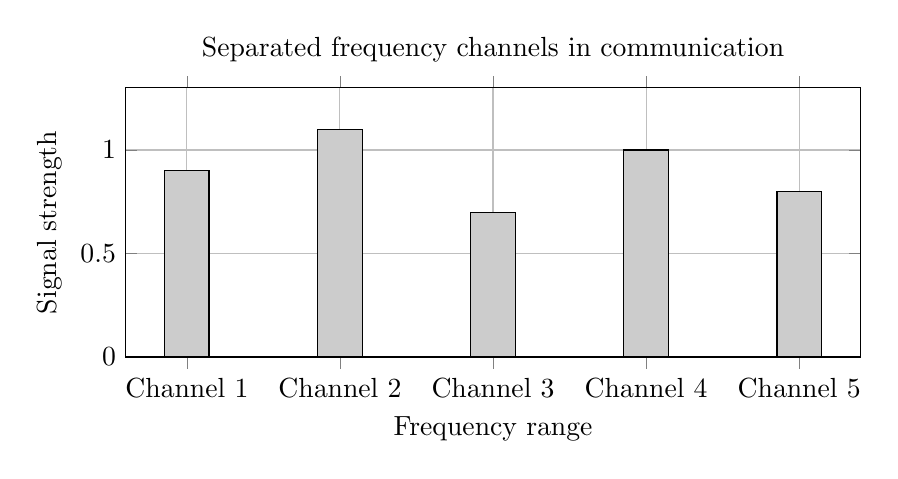
\begin{tikzpicture}
		\begin{axis}[
			width=0.9\textwidth,
			height=5cm,
			ybar,
			bar width=16pt,
			xlabel={Frequency range},
			ylabel={Signal strength},
			ymin=0,
			ymax=1.3,
			xtick={1,2,3,4,5},
			xticklabels={Channel 1,Channel 2,Channel 3,Channel 4,Channel 5},
			grid=both,
			title={Separated frequency channels in communication}
			]
			
			\addplot[
			fill=gray!40,
			draw=black
			]
			coordinates {
				(1,0.9)
				(2,1.1)
				(3,0.7)
				(4,1.0)
				(5,0.8)
			};
			
		\end{axis}
	\end{tikzpicture}
	\caption{
		Several signals can be transmitted separately over different frequency ranges
		and later filtered out again.
	}
	\label{fig:frequenzkanaele}
\end{figure}

Another important point is the separation of signal and disturbance.

Real transmission systems always contain noise,
reflections,
or other disturbances.
Frequency analysis makes it possible to recognize
which components belong to the desired signal
and which should be weakened or filtered out.

Without such mathematical methods,
modern data transmission,
mobile communication,
Wi-Fi,
satellite communication,
and fiber-optic technology would hardly be conceivable.

\begin{NoteBox}[Fourier analysis as a foundation of the digital world]
	\small
	\label{box:fourier-digitale-welt}
	The modern information society is based on the processing of signals.
	
	Whether Wi-Fi,
	mobile communication,
	satellite links,
	or fiber-optic technology:
	frequencies must be analyzed,
	separated,
	filtered,
	and reconstructed everywhere.
	
	Fourier analysis is therefore one of the mathematical foundations
	of modern communication.
\end{NoteBox}

Fourier analysis shows particularly clearly here
that abstract mathematics has immediate technological significance.

It makes it possible
to transmit information reliably,
reduce disturbances,
and process many data streams simultaneously.

% ============================================================
\subsection{Fourier Analysis and the Structure of the World}

Fourier analysis shows in an impressive way
that simple mathematical patterns are often hidden behind complex phenomena.

What at first appears chaotic,
irregular,
or incomprehensible
can often be described by the superposition of elementary oscillations.

This applies to music,
images,
electrical signals,
medical measurement data,
light spectra,
and even wave functions in quantum mechanics.

The same mathematical idea appears everywhere:
complexity arises from the combination of simple structures.

Fourier analysis therefore provides a particularly strong example
of the central guiding idea of this book:

\begin{NoteBox}[Mathematical order behind complex phenomena]
	\small
	\label{box:fourier-mathematische-ordnung}
	The world often appears complicated and chaotic.
	
	Yet behind many phenomena there is
	a deep mathematical structure.
	
	Fourier analysis shows
	that even complex signals
	can be traced back to simple oscillations.
\end{NoteBox}

Mathematics is therefore not merely a calculating tool,
but a language
with which hidden order can be made visible.

Fourier theory does not create this order --
it discovers it.

This is precisely where the close connection
between mathematics and reality becomes visible.

Fourier analysis makes clear
that nature does not consist of isolated individual phenomena,
but of superimposed structures
that can be described mathematically.

Mathematics thereby becomes a key
for deciphering the hidden structure of the world.